% ****** Start of file aipsamp.tex ******
%
%   This file is part of the AIP files in the AIP distribution for REVTeX 4.
%   Version 4.1 of REVTeX, October 2009
%
%   Copyright (c) 2009 American Institute of Physics.
%
%   See the AIP README file for restrictions and more information.
%
% TeX'ing this file requires that you have AMS-LaTeX 2.0 installed
% as well as the rest of the prerequisites for REVTeX 4.1
%asd
% It also requires running BibTeX. The commands are as follows:
%
%  1)  latex  aipsamp
%  2)  bibtex aipsamp
%  3)  latex  aipsamp
%  4)  latex  aipsamp
%
% Use this file as a source of example code for your aip document.
% Use the file aiptemplate.tex as a template for your document.
\documentclass[%
9pt,
 aip,
%jmp,%
%bmf,%
%sd,%
rsi,%
 amsmath,amssymb,
preprint,%
%reprint,%
%author-year,%
%author-numerical,%
]{revtex4-1}

\usepackage{graphicx}% Include figure files
\usepackage{dcolumn}% Align table columns on decimal point
\usepackage{bm}% bold math
%including for citations
\usepackage{xr}
\externaldocument{MainPart}
%\usepackage[outdir=./plots/]{epstopdf}


% \usepackage[utf8]{inputenc}
% \usepackage{amssymb,amsmath}
 % \usepackage{diagbox}
% \usepackage{tabularx}
% \usepackage{xcolor}
 \graphicspath{ {plots/} }
 %\DeclareGraphicsExtensions{.}

%\usepackage[mathlines]{lineno}% Enable numbering of text and display math
%\linenumbers\relax % Commence numbering lines

% %%%%%%%%%%%%%%%%%%%%%%%%%%%%%%%%%%%%%%%%%%%%%%%%%%%%%%%%%%%%%%%%%%%%%%%%%%
% % Karin: Egor, this helps me to interact with you in the manuscript
% % you may find
% %   \InTextCommment{KZ}{my comment}
% %   \todo{what to do}
% % FOR AUTHORS COMMENTS! REMOVE FROM HERE.....

% %\usepackage{multicol}
% %\setlength{\columnsep}{1cm}

 \usepackage[export]{adjustbox}
 \usepackage{ulem}
 \usepackage{anyfontsize}
 \usepackage[textwidth=1.2cm,textsize=tiny]{todonotes}
 \setlength{\marginparwidth}{1cm}

% % long comment
 \newcommand{\InTextComment}[2]{
 	%\renewcommand{\baselinestretch}{1.0} 
 	\textcolor{blue}{\textsf{{\footnotesize \textbf{- #1:} #2 -}}}\newline
 	%\renewcommand{\baselinestretch}{1.5} 
 }
 
% % UP TO HERE, BEFORE SUBMISSION
% %%%%%%%%%%%%%%%%%%%%%%%%%%%%%%%%%%%%%%%%%%%%%%%%%%%%%%%%%%%%%%%%%%%%%%%%%%

% KZ: activate for aiding reading
%\usepackage{helvet}
%\renewcommand{\familydefault}{\sfdefault}
%\fontsize{8}{11}\selectfont
\renewcommand{\baselinestretch}{1.2} %2.0

%defining dimensions

\newcommand{\thermalconductivity}{$\mathrm{W m^{-1} K^{-1}}$}
\newcommand{\hcoefficient}{$\mathrm{W m^{-2} K^{-1}}$}
\newcommand{\mobility}{$\mathrm{m^{2} V^{-1} s^{-1}}$}

\begin{document}


\section*{Supporting information.}

\addtocounter{figure}{5}
\addtocounter{equation}{11}

\subsection*{General analytic solution for the steady-state 1D heat equation}
% \begin{figure}
% 	\centering
% 	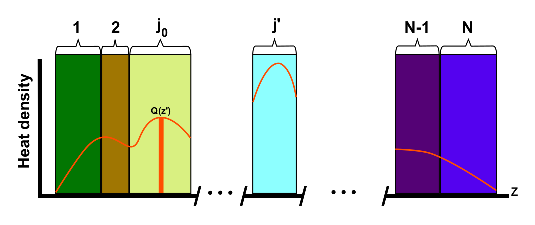
\includegraphics[width=0.4\textwidth]{General_plots_3}
% 	\caption{Discretization for solving the 1D heat equation for multiple layers. The orange line indicates the heat density distribution $Q(z)$. The top labels enumerate the layers, each of which has its own thermal conductivity $\kappa_{j'}$ and thickness $L_{j'}$. }
% 	\label{fig:MultiLayersSetup}
% \end{figure}


Utilizing a thermal conductivity function, in which a thermal conductivity $\kappa_j$ is assigned to each layer $j$ located along the $z$-axis (cf. Fig.~\ref{fig:MultiLayersSetup}), we can formulate a heat equation for the whole device.
The general solution of the differential equation (\ref{eq:1Dheatequation}) is given by a Green function $G(z,z_0)$ that solves Eq.~(\ref{eq:GreenFunctionEquation}). 

\begin{equation}
-\left( \kappa(z) G_z'(z,z_0)  \right)_z' = \delta(z-z_0)
\label{eq:GreenFunctionEquation}
\end{equation}

If one multiplies Eq.~(\ref{eq:GreenFunctionEquation}) by $H(z_0)$ and integrates it with respect to $z_0$, one obtains the following equation: %. 
\begin{equation}
-{\left(\kappa (z) \left(\int_0^L dz_0 G(z,z_0) H(z_0) \right)_z' \right)}_z' = H(z).
\label{eq:GreenFunctionHeatEquation}
\end{equation}

Therefore, the term in the inner bracket of Eq.~(\ref{eq:GreenFunctionHeatEquation}) should be equal to the $T(z)$ in the presence of the heat distributed as $H(z)$. 

If one returns to the equivalent notation with several layers and imposes the preservation of heat flux across the interfaces, one arrives at the equation: %.
\begin{equation}
T(z) = \sum_{j'=1}^{N} \int_{z_{j'-1}}^{z_{j'}} H(z_0) G(z,z_0) dz_0.
\label{eq:GreenFunctionSolution}
\end{equation}

Where $z_{j'}=\sum_{i=1}^{j'} L_i$ and $L_{i}$ refers to the thickness of the individual layers.
The Greens function $G(z,z_0)$ can then be conveniently written using functions $W^L(z)$ and $W^R(z)$ for each layer $b$:%in equations \ref{eq:greenfunction}.

% \begin{subequations}
% 	 \begin{align}
% 		W_b^L(z) =& \frac{1}{h_L}+\sum_{i=1}^{b-1} \frac{L_i}{\chi_i} + \frac{z}{\chi_b} \label{eq:WL}\\
%         W_b^R(z) =& \frac{1}{h_R}+\sum_{i=b+1}^{N} \frac{L_i}{\chi_i} + \frac{L_b - z}{\chi_b} \label{eq:WR}\\
%         G_{j,j'}^L =& \frac{1}{\sum_{i=1}^{N} \frac{L_i}{\chi_i}} W^L_{j}(z) W^R_{j'}(z'), z<z' \label{eq:GL}\\
%         G_{j,j'}^R =& \frac{1}{\sum_{i=1}^{N} \frac{L_i}{\chi_i}} W^R_{j}(z) W^L_{j'}(z'), z>z' \label{eq:GR}
% 	\end{align}
%     \label{eq:greenfunction}
% \end{subequations}

\begin{subequations}
    \begin{align}
    W_b^L(z) =& \frac{1}{h_L}+\sum_{i=1}^{b-1} \frac{L_i}{\chi_i} + \frac{-\left( \sum_{i=1}^{b-1} L_i \right) + z}{\chi_b} \label{eq:WL}\\
    W_b^R(z) =& \frac{1}{h_R}+\sum_{i=b+1}^{N} \frac{L_i}{\chi_i} + \frac{\left( \sum_{i=1}^{b} L_i \right)  - z}{\chi_b}. \label{eq:WR}\\
    \end{align}
    \label{eq:Wfunction}
\end{subequations}

Then, the Green's functions $G^{L}(z,z_0)$ for $z<z_0$ and $G^{R}(z,z_0)$ for $z>z_0$ read:

\begin{subequations}
    \begin{align}
    G_{j,j'}^L =& \frac{1}{\sum_{i=1}^{N} \frac{L_i}{\chi_i}} W^L_{j}(z) W^R_{j'}(z_0), \quad \mathrm{for~} z<z_0 \label{eq:GL}\\
    G_{j,j'}^R =& \frac{1}{\sum_{i=1}^{N} \frac{L_i}{\chi_i}} W^R_{j}(z) W^L_{j'}(z_0), \quad \mathrm{for~} z>z_0. \label{eq:GR}
    \end{align}
    \label{eq:greenfunction}
\end{subequations}

While $j$ and $z$ are the coordinates of the layer where one calculates temperature, $j'$ and $z_0$ correspond to that layer from which one want to calculate contribution to the temperature (cf.~Figure \ref{fig:MultiLayersSetup}). 
To obtain temperature distribution in certain layer $j$ at point $z$ for given heat distribution $H(z_0)$ according to Eq.~(\ref{eq:GreenFunctionSolution}), one should integrate $H(z_0)$ weighted with the corresponding Green function $G_{j,j'}(z,z_0)$ with respect to $z_0$ and sum the contributions from all layers $j'$ . 

\subsection*{Testing the consistency of the analytical model with simulation results.}

The maximum temperature predicted by the simplified Eq.~(\ref{eq:TmaxAsAFunctionOfIVErec}) corresponds well to the prediction of the full simulation for a large range of heat transfer coefficients.
Figure~\ref{fig:connection_to_experiment} shows the relative error,
$\frac{|T_{max,an} - T_{max,sim}| }{T_{max,sim}-300K} - 1$, between $T_{max}$ either predicted on the basis of Eq.(\ref{eq:TmaxAsAFunctionOfIVErec}) and the current obtained from the simulation ($T_{max,an}$) and $T_{max}$ directly obtained from the simulations ($T_{max,sim}$).

%----------------------------
% push into SUI
\begin{figure}[h]
    \centering
    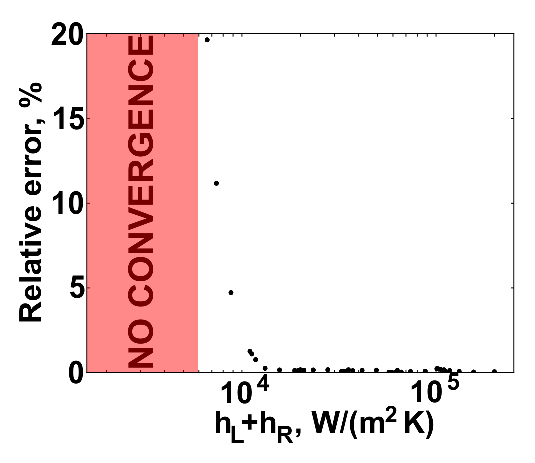
\includegraphics{General_plots_2.eps}
    \caption{Validity of the maximum temperature predicted by Eq.(\ref{eq:TmaxAsAFunctionOfIVErec}) as a function of the total heat transfer coefficient $h_L + h_R$. Shown is the relative error $\frac{|T_{max,an} - T_{max,sim}| }{T_{max,sim}-300K} - 1$ formed between $T_{max,sim}$ deduced from the full simulation and $T_{max,an}$ predicted from Eq.(\ref{eq:TmaxAsAFunctionOfIVErec}) using only the current obtained from the simulation. In the red shaded region, located at small $h_L + h_R$, the device overheats so that the simulations do not converge.}
    \label{fig:connection_to_experiment}
\end{figure}
%----------------------------------------

For $h_L + h_R < 4\cdot10^3$~\hcoefficient~, $T_{max,sim}$ cannot be determined, because thermal runaway prevents the convergence to a steady state (red shading).
Solely closely above the thermal runaway region, $h_L + h_R < 10^4$~\hcoefficient~, the temperature predicted by Eq.(\ref{eq:TmaxAsAFunctionOfIVErec}) deviates from the simulation. The prediction of Eq.(\ref{eq:TmaxAsAFunctionOfIVErec}) fails for these heat transfer coefficients, because the temperature distribution in the device is not uniform.

%It can be successfully used to determine how much the device will heat up under particular electric current and all other terms in this equation are accessible through experiment. 


\subsection*{Feedback between heat transport and device temperature.}

Here we intend to identify for which $h$ and $\kappa$ it is safe to assume that the heat transport away from the electrically active region does not affect the temperature of this region. 
For situations in which this assumption is invalid, we want to gather the symptoms of the electro-thermal feedback.
We check for the presence of an electro-thermal feedback by comparing the temperature distribution $T_{sim}(z)$ from the full simulation and $T_{an}(z)$ from solving the steady state heat transport equation, Eq.~(\ref{eq:1Dheatequation}).
Eq.~(\ref{eq:1Dheatequation}) is inherently unable to account for a possible feedback of the heat transport on the charge transport and the heat generation profile.
Hence, we can interpret any deviation of $T_{an}(z)$ from $T_{sim}(z)$ as a manifestation of a feedback.

Such a comparison is particularly feasible for our symmetric model OLED.
As the temperature distribution is symmetric, the largest temperature $T_{max}$ is always established in the device center (cf. Fig.~\ref{fig:setup}-c). Rather than accounting for the entire profiles $T(z)$,
it is sufficient to compare the predicted maxima $T_{max,an}$ and $T_{max,sim}$.
%Such a comparison is particularly feasible for our symmetric model OLED.
%As the temperature distribution is symmetric and the largest temperature $T_{max}$ is always established in the device center (cf. Fig.~\ref{fig:setup}-c), it is sufficient to compare the predicted $T_{max,an}$ and $T_{max,sim}$.
For sufficiently large $\kappa$ and $h$, we expect that the heat flow is large enough to prevent any heat accumulation in the electrically active region. 
Hence, the heat density profile $H(z)$ is independent of $\kappa$ and $h$. %and is solely governed by the electric properties and operating conditions.
Guided by Fig.~\ref{fig:I-Vandh-k-maxT}-b, we encounter this situation for $\kappa = 1$~\thermalconductivity~ and $h = 10^5$~\hcoefficient~ at an operating voltage of 5~V.  
The simulated heat density profile $H(z)$ retrieved for these thermal parameters gives rise to the total heat $H_{tot} = \int_0^L dz H(z)$. 
Since this $H(z)$ is solely governed by the electric properties and operating conditions, it will now serve as the input for Eq.~(\ref{eq:1Dheatequation}) to inspect $T_{an}$ for other values of $\kappa$ and $h$.

\begin{figure}
    \centering
    \includegraphics[width=0.75\textwidth]{General_plots_5.pdf}
    \caption{(a) Maximum temperature $T_{max,sim}$ (black) and $T_{max,an}$ (red) in the device as a function of the heat transfer coefficient $h$ at $\kappa$=1~\thermalconductivity. $T_{max,sim}$ are temperature values extracted from simulations of the model OLED operated at 5~V. $T_{max,an}$ are temperature values calculated from the analytical solution of Eq.~(\ref{eq:1Dheatequation}) using the heat generation profile obtained for $h=10^5$~\hcoefficient. (b) Relative increase in temperature, $\frac{T_{max,sim}}{T_{max,an}}-1$, (left axis) compared to the total device heat $H_{tot}$ (right axis) as a function of the h-coefficient. (c) Maximum temperature $T_{max,sim}$ (black) and $T_{max,an}$ (red) in the device (left axis) and $H_{tot}$ (right axis) as a function of thermal conductivity at h = $10^{4.25}$~\hcoefficient. (d) Local changes in heat density due a change in a thermal parameter. $\frac{H_{h}(z)}{H_{h_{ref}}(z)}-1$ monitors the relative change in heating density when going from $h = 10^{3.5}$ to $10^5$~\hcoefficient at $\kappa$ = 1~\thermalconductivity (black curve) and $\frac{H_{\kappa}(z)}{H_{\kappa_{ref}}(z)}-1$ the relative change in heat density in going from
        $\kappa = 1$ to $10^{-4}$~\thermalconductivity~for $h$ = $10^{4.25}$~\hcoefficient (red curve).}
    \label{fig:final4plots}
\end{figure}

Figure~\ref{fig:final4plots}-a shows the evolution of $T_{max,an}$ and $T_{max,sim}$ for varying heat transfer coefficients $h$ at $\kappa = 1$~\thermalconductivity. 
As long as $T_{max}$ remains smaller than 310~K, $T_{max,an}$ (red) and $T_{max,sim}$ (black) are indistinguishable.
Below $h \approx 10^4$~\hcoefficient, the simulations reveal a markedly larger temperature as one would expect from the analytical solution $T_{max,an}$. 
Not only the two temperatures $T_{max,sim}$ and $T_{max,an}$, but also the trend in the deviation between the two temperatures, cast for convenience into the expression $\frac{T_{max,sim}}{T_{max,an}}-1$ in Fig.~\ref{fig:final4plots}-b, is directly related to the total amount of heat $H_{tot}$ (orange) produced in the device.
Hence, the elevated temperature $T_{max,sim}$ is the symptom for the electro-thermal feedback between the transported heat and the heat density profile that causes self-heating.

Note that the equality between $T_{max,sim}$ and $T_{max,an}$ does not necessarily imply the absence of electro-thermal feedback. 
To illustrate that, Fig.~\ref{fig:final4plots}-c shows $T_{max,sim}$ and $T_{max,an}$ as a function of $\kappa$ at constant $h = 10^{4.25}$~\hcoefficient. 
At the first glance, $T_{max,sim}$ and $T_{max,an}$ coincide even for lowest probed $\kappa = 10^4$~\thermalconductivity.
%the heat transfer equation appears to correctly predict the maximum temperature in the OLED even for very low $\kappa = 10^4$~\thermalconductivity.
However, a closer inspection of the situation at such low $\kappa$ reveals that there is nevertheless an electro-thermal feedback and, hence, heat accumulation inside the electrically active layers.
This accumulation of heat predominantly changes the \textit{shape} of the heat density profile $H(z)$.
%To visualize this change shape, we plot the relative change of heat density, $\frac{H_{\kappa}(z)}{H_{\kappa_{ref}}(z)}-1$ (red curve), that occurs upon going from $\kappa$ = 1 (reference) to $10^{-4}$~\thermalconductivity, as a function of the position $z$ in the electrically active region in Fig.~\ref{fig:final4plots}-d.
To visualize how the heat density $H(z)$ differs in each position $z$ in the electrically active region between $10^{-4}$~\thermalconductivity and $\kappa$ = 1~\thermalconductivity, we plot the corresponding relative change of heat density, $\frac{H_{\kappa}(z)}{H_{\kappa_{ref}}(z)}-1$ (red curve) in Fig.~\ref{fig:final4plots}-d.
%While the heat produced at the organic-organic interface is not affected by $\kappa$.
%
%Lowering $\kappa$ leads to an enhanced heating closer to the surfaces. This additional heat diffuses more easily to the surfaces that to the center due to the non-uniform temperature distribution across the device. 
%This change in heat density does not occur uniformly across the device, but is rather V-shaped.
%Due to the arc-shaped temperature distribution across the OLED, the lowering of $\kappa$ causes the temperature to rise mainly in the center of the device and to a much lesser extent near the outer surfaces. 
This change in heat density does not occur uniformly across the active layers. 
Rather, regions are heated the stronger the closer they are to the surface.
Due to the arc-shaped temperature distribution across the within the active layers, a lowering of $\kappa$ causes the temperature to rise mainly in the center of the device and, to a much lesser extent, near the outer surfaces. 
While the temperate elevation increases the recombination and the electric conductivity at the device center, the electrical conductivity near the surfaces considerably lesser raised.
Since Joule heating is more pronounced in the regions with lower electrical conductivity, more heat is produced near the surface compared in the center.
%The correspondingly occurring V-shape  
%Temperature increases mainly in the middle of the device which in turn increases recombination and overall electric current. On the other hand, temperature close to surfaces is smaller and resistivity of layers is higher there. So, comparing heating in the center and close to surfaces, Joule heating is higher in the regions with low electrical conductivity. From the equation \ref{eq:analtmax} one can easily deduce that such changes in the shape affect maximum temperature and this is exactly what we see here.

For comparison, we also show that shape of the heat density profile $H(z)$ is essentially preserved when comparing excellent ($h$ = $10^{5}$~\hcoefficient) and inferior ($10^{3.5}$~\hcoefficient) heat transfer with the environment.
Fig.~\ref{fig:final4plots}-d (black curve) shows the corresponding relative change of heat density, $\frac{H_{h}(z)}{H_{h_{ref}}(z)}-1$.
Throughout the active layers, this change is practically uniform except for sudden increase in the close vicinity of the outer surfaces. The overall temperature profile is governed by these extended regions of uniform heating; the very narrow surface regions do not have a perceivable impact.


%Such enhanced heating contributions near the surface play a sub-ordinate role in establishing the temperature as these surface regions are small compared to the regions of uniform heating.

%Note that relative change appears to There are no real physical consequences for the device, because heating density in this region is small compared to other regions in the device and hard to notice absolute changes look substantial on relative scale. 
%We see that changing h-coefficient uniformly increases heating all across the device. 

%In this section we want to provide some overview how equations \ref{eq:analt} work in detail. We start investigation from taking a look on how heat transport coefficient affects temperature distribution. The whole system reacts to its change via complex mechanisms, therefore we are particularly interested when we can make simple conclusions from change in the device thermal structure and when they stop working. We start this investigation from fixing thermal conductivity and changing heat transport coefficient. This attempt is depicted in Figure \ref{fig:final4plots}-a. 

%\begin{figure}
%	\centering
%	\includegraphics[width=0.5\textwidth]{Graph2}
%	\caption{Maximum temperature in the device as a function of h-coefficient at point $\kappa$=1 W/(mK). Simulated temperatures are temperatures extracted from our simulations. Predicted temperatures are temperatures calculated from analytical model using first two points as reference ones.}
%	\label{fig:h-maxT-appmaxT}
%\end{figure}

%As one can see, reverse proportion rule of Eq. \ref{eq:analt} works until certain limit, roughly speaking, until around 310~K. After that, simulated temperature numbers diverge quickly from the predicted values. The difference of course comes from $H_{uni} x$ term, which corresponds to the total amount of heat generated in the device. The total generated heat as well as relative difference between two temperatures as a function of h are presented at Figure \ref{fig:final4plots}-b. 

%\begin{figure}
%	\centering
%	\includegraphics[width=0.5\textwidth]{Graph3}
%	\caption{Difference between relative temperature and total device heating.}
%	\label{fig:h-dT-H}
%\end{figure}

%From this one can easily see that most difference between equation \ref{eq:analtmax} and simulation comes from our ignorance about how the amount of generated heat depends on the change of h. We can see that when h-coefficient decreases, temperature rises by two mechanisms. First is the change of temperature due to less efficient heat outflow. But that temperature rise produces via electro-thermal coupling another effect of increased device heating. 

%With thermal conductivity the results are completely different, Figure \ref{fig:final4plots}-c. Suddenly, analytical model predicts the maximum temperature behavior very well in any region. Moreover, it even overestimates the result which was not the case with heat transport coefficient. The only way to understand it via analytic model is the second order term proportional to $x$ in the brackets. As the heating profile shrinks, it leads to the changes in temperature which are not governed by total heating. To look at that in more details we compared how heating profiles locally changes when we change separately heat transport coefficient and thermal conductivity. Results are presented at Figure \ref{fig:final4plots}-d

%\begin{figure}
%	\centering
%	\includegraphics[width=0.5\textwidth]{Graph5}
%	\caption{Maximum temperature in the device as a function of thermal conductivity at point h=17782 W/($m^2$K) (This corresponds to h=$10^{4.25}$). Simulated temperatures are temperatures extracted from our simulations. Predicted temperatures are temperatures calculated from analytical model using first two points as reference ones.}
%	\label{fig:k-maxT-appmaxT-H}
%\end{figure}

%So we see that the total device heating depends differently on thermal conductivity than on h-coefficient. The absolute values on this plot are not important, what we are looking for is the shape. Also, on the h-coefficient curve on can see that the edges are very much lifted up. There are no real physical consequences for the device, because heating density in this region is small compared to other regions in the device and hard to notice absolute changes look substantial on relative scale. 

%We see that changing h-coefficient uniformly increases heating all across the device. At the same time, changes of thermal conductivity lead to heating which is more profound close to the surfaces and therefore is easier to diffuse to the edge. This is the consequence of non-uniform temperature distribution across the device. Temperature increases mainly in the middle of the device which in turn increases recombination and overall electric current. On the other hand, temperature close to surfaces is smaller and resistivity of layers is higher there. So, comparing heating in the center and close to surfaces, Joule heating is higher in the regions with low electrical conductivity. From the equation \ref{eq:analtmax} one can easily deduce that such changes in the shape affect maximum temperature and this is exactly what we see here.

%\begin{figure}
%	\centering
%	\includegraphics[width=0.5\textwidth]{Graph7}
%	\caption{How local heating changes when one varies h-coefficient (black curve) or thermal conductivity (red curve). Black curve: $\kappa$ = 1 W/(mK), h-coefficient varies from $10^{3.5}$ to $10^5$ Red curve: h = $10^{4.25}$, $\kappa$ varies from $10^{-4}$ to 1. }
%	\label{fig:z-hdH-kdH}
%\end{figure}

% \begin{table}[]
% \makebox[\textwidth]{\begin{tabular}{|c|c|c|c|c|c|c|c|c|c|c|}
% \hline
% \diagbox{h}{$\kappa$}      & 0.0001 & 0.000316 & 0.001 & 0.00316 & 0.01  & 0.0316 & 0.1   & 0.316 & 1    & 3.16 \\\hline
% 1000   &\cellcolor{black!100}&\cellcolor{black!100}&\cellcolor{black!100}&\cellcolor{black!100}&\cellcolor{black!100}&\cellcolor{black!100}&\cellcolor{black!100}&\cellcolor{black!100}&\cellcolor{black!100}&\cellcolor{black!100}\\\hline
% 1780   &\cellcolor{black!100}&\cellcolor{black!100}&\cellcolor{black!100}&\cellcolor{black!100}&\cellcolor{black!100}&\cellcolor{black!100}&\cellcolor{black!100}&\cellcolor{black!100}&\cellcolor{black!100}&\cellcolor{black!100}\\\hline
% 3160   &\cellcolor{black!100}&\cellcolor{black!100}&\cellcolor{black!100}&\cellcolor{black!100}&\cellcolor{black!100}&\cellcolor{black!100}&\cellcolor{black!100}&\cellcolor{red!25}1.26&\cellcolor{red!25}1.26&\cellcolor{red!25}1.25\\\hline
% 5620   &\cellcolor{black!100}&\cellcolor{green!25}0.94&\cellcolor{green!25}0.97&\cellcolor{green!25}0.99&\cellcolor{green!25}0.99&\cellcolor{green!25}0.99&\cellcolor{green!25}0.99&\cellcolor{green!25}1.01&\cellcolor{green!25}1.01&\cellcolor{green!25}1.01\\\hline
% 10000  &\cellcolor{black!100}&\cellcolor{green!25}0.92&\cellcolor{green!25}0.96&\cellcolor{green!25}0.98&\cellcolor{green!25}0.99&\cellcolor{green!25}0.99&\cellcolor{green!25}0.99&\cellcolor{green!25}1.00&\cellcolor{green!25}1.00&\cellcolor{green!25}1.00\\\hline
% 17800  &\cellcolor{yellow!25}0.89&\cellcolor{green!25}0.90&\cellcolor{green!25}0.94&\cellcolor{green!25}0.97&\cellcolor{green!25}0.99&\cellcolor{green!25}0.99&\cellcolor{green!25}0.99&\cellcolor{green!25}1.00&\cellcolor{green!25}1.00&\cellcolor{green!25}1.00\\\hline
% 31600  &\cellcolor{yellow!25}0.88&\cellcolor{yellow!25}0.89&\cellcolor{green!25}0.92&\cellcolor{green!25}0.96&\cellcolor{green!25}0.98&\cellcolor{green!25}0.99&\cellcolor{green!25}0.99&\cellcolor{green!25}1.00&\cellcolor{green!25}1.00&\cellcolor{green!25}1.00\\\hline
% 56200  &\cellcolor{yellow!25}0.87&\cellcolor{yellow!25}0.87&\cellcolor{green!25}0.90&\cellcolor{green!25}0.94&\cellcolor{green!25}0.97&\cellcolor{green!25}0.99&\cellcolor{green!25}0.99&\cellcolor{green!25}1.00&\cellcolor{green!25}1.00&\cellcolor{green!25}1.00\\\hline
% 100000 &\cellcolor{yellow!25}0.87&\cellcolor{yellow!25}0.87&\cellcolor{yellow!25}0.89&\cellcolor{green!25}0.92&\cellcolor{green!25}0.96&\cellcolor{green!25}0.98&\cellcolor{green!25}0.99&\cellcolor{green!25}1.00&\cellcolor{green!25}1.00&\cellcolor{green!25}1.00   \\\hline

% \end{tabular}}
% \caption{Comparision between simulation results and results predicted from equation \ref{eq:TmaxAsAFunctionOfIVErec}. Numbers presented correspond to simulated temperature divided by predicted (both measured relative to the the ambient temperature). Green cell color - error is less than 10\%, yellow - more than 10\% and less than 25\%, red - more than 25\%. Black cell marks simulations with such parameters that simulation did not converged. }
% \label{tab:ComparationSimToPredicted}
% \end{table}

\end{document}
